% !TeX root = ../main.tex

La necessità di progettare e realizzare un servizio di conversione in modo tale che possa essere eseguito on-demand (e in modo automatico) deriva sia dalla quantità di documenti già archiviati in formato PDF (circa 2200) sia dalla loro eterogeneità. Su 2200 documenti infatti, circa 200 sono libri e i restanti sono riviste. Le riviste, rispetto i libri, contengono elementi all'interno di ogni pagina che rendono molto complicata la loro conversione.\\
Dati i formati in input (PDF o HTML) e stabilito il formato di output (EPUB) è necessario definire i tool e la procedura di conversione. Prima di analizzare eventuali librerie utili a implementare la procedura di conversione è stata effettuata una ricerca di tool già disponibili sul mercato in grado di svolgere il compito richiesto. I principali requisiti per la ricerca del tool sono:
\begin{itemize}
    \item possibilità di convertire da almeno uno dei due formati disponibili in input verso il formato di output,
    \item eseguibile binario senza GUI.
\end{itemize}

\section{Calibre}
Software libero, open source\footnote{\url{https://github.com/kovidgoyal/calibre}} e multipiattaforma, fornisce una suite di tool creare, conservare, catalogare e manipolare eBook. Tra i formati supportati, sia in input che output, è possibile trovare Epub, Fb2, Html, Lit, Mobi, Odt e Pdf.\\
Tra i vari tool della suite è presente un convertitore, chiamato \textit{ebook-convert}\footnote{\url{https://manual.calibre-ebook.com/generated/en/ebook-convert.html}}, il quale soddisfa i requisiti sopra indicati.

\begin{listing}[H]
\begin{minted}{bash}
brew install calibre
ebook-convert test.pdf test.epub
\end{minted}
\caption{Esempio: Installazione Calibre e conversione base PDF/EPUB tramite \textit{ebook-convert}}
\end{listing}

% descrivere i test di conversione fatti, perchè le conversioni html2epub fanno schifo (e quindi si fa pdf2epub)

\section{Progettazione}
Si descrive in questa sezione come è stato progettato e sviluppato il servizio \textit{pdf2epub} dato il tool \textit{ebook-convert} (suite Calibre), scelto come meccanismo core per la conversione da PDF a EPUB.\\
L'approccio adottato consiste nello sviluppo di un "wrapper" del tool \textit{ebook-convert} in modo da fornire le sue funzionalità attraverso una REST API.\\
L'unica funzione che deve essere svolta da \textit{pdf2epub} è: dato un documento in formato PDF in input, restituire in output quel documento convertito in formato EPUB. Per questo motivo si identifica un unico endpoint, il quale deve fornire la possibilità di passare tutti i parametri necessari alla configurazione della conversione. Tali parametri corrispondono agli argomenti\footnote{\url{https://manual.calibre-ebook.com/generated/en/ebook-convert.html}} accettati dall'eseguibile \textit{ebook-convert}:
\begin{itemize}
    \item \textbf{Global} - Opzioni comuni a qualsiasi tipo di conversione.
    \item \textbf{Look and Feel} - Opzioni per controllare l'aspetto grafico dell'output.
    \item \textbf{Heuristic Processing} - Opzioni per modificare il testo e la struttura del documento utilizzando pattern comuni.
    \item \textbf{Search and Replace} - Opzioni per modificare il testo e la struttura del documento utilizzando i modelli definiti dall'utente.
    \item \textbf{Structure Detection} - Opzioni per il controllo del rilevamento automatico della struttura del documento.
    \item \textbf{Table of Contents} - Opzioni per il controllo della generazione dell'indice.
    \item \textbf{Metadata} - Opzioni per impostare i metadati nell'output.
    \item \textbf{Debug} - Opzioni di debug.
    \item \textbf{Input PDF} - Opzioni specifiche per il documento di input in formato PDF.
    \item \textbf{Output EPUB} - Opzioni specifiche per il documento di output in formato EPUB.
\end{itemize}
L'unico endpoint implementato è chiamato \textit{convert} con metodo \textit{POST}: esso richiede come unico parametro obbligatorio il file pdf da convertire oltre ai parametri opzionali sopra indicati. Ogni chiamata consiste nella esecuzione di un task tramite un \textit{ThreadPoolExecutor} il quale fa uso del componente \textit{EbookConverter}. Tale entità rappresenta il vero e proprio "wrapper" dell'eseguibile \textit{ebook-convert} fornito da Calibre.
\begin{figure}[H]
\centering
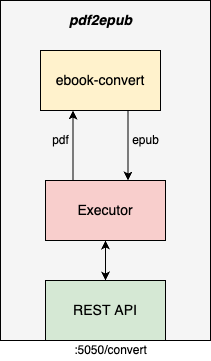
\includegraphics[width=0.25\textwidth]{img/tesi-4-pdf2epub.drawio.png}
\caption{Architettura servizio pdf2epub}
\end{figure}
\begin{figure}[H]
\centering
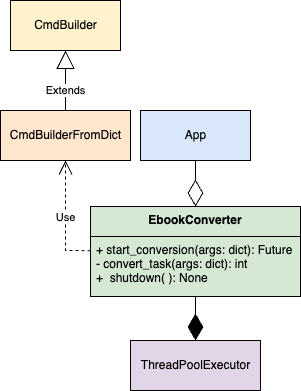
\includegraphics[width=0.6\textwidth]{img/tesi-5-pdf2epub.drawio.png}
\caption{Diagramma delle classi: pdf2epub}
\end{figure}

\subsection{Delivery pdf2epub}
La modalità di delivery scelta per il servizio \textit{pdf2epub} è tramite immagine Docker rilasciata sul container registry aziendale \textit{psacr}, per il quale si fa uso dei servizi cloud forniti da Azure\footnote{\url{https://azure.microsoft.com/en-us/services/container-registry/\#overview}}.\\
La regola che attiva la pipeline di rilascio è definita sul push di un tag sul branch principale (\textit{main}). In questo caso vengono caricate sul container registry due nuove immagini: ($i$) una con il tag esplicito che si aggiunge alle altre già caricate e ($ii$) un'altra con il tag \textit{latest}, la quale sovrascrive l'ultima immagine \textit{latest} mantenedola aggiornata all'ultima versione.
\begin{figure}[H]
\centering
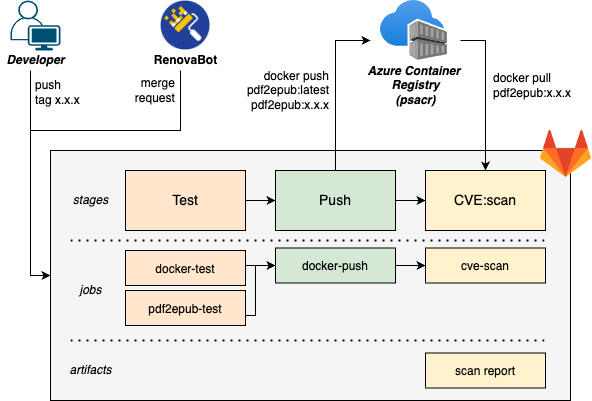
\includegraphics[width=0.9\textwidth]{img/tesi-6-pdf2epub.drawio.png}
\caption{Continuous Integration/Delivery pdf2epub}
\end{figure}
L'immagine Docker del servizio è costruita utilizzando come base di partenza l'immagine \textit{linuxserver/calibre}\footnote{\url{https://hub.docker.com/r/linuxserver/calibre}}. Questa scelta è data dalle seguenti motivazioni/vantaggi:
\begin{itemize}
    \item \textit{LinuxServer.io}\footnote{\url{https://www.linuxserver.io/}} è una community grande e attiva che distribuisce e mantiene tantissime immagini largamente diffuse,
    \item l'installazione e la manutenzione all'interno di un container di Calibre, ebook-convert e di tutte le dipendenze è rimandata alla community che gestisce l'immagine Docker,
    \item tramite l'utilizzo di un tool per l'aggiornamento automatico delle dipendenze, in questo caso specifico Renovate\footnote{\url{hhttps://github.com/renovatebot/renovate}}, l'aggiornamento di Calibre, di ebook-convert e delle dipendenze è semplificato e automatizzato.
\end{itemize}
\begin{listing}[H]
\begin{minted}{docker}
FROM --platform=linux/amd64 linuxserver/calibre:5.43.0

WORKDIR /home/pdf2epub

ENV FLASK_DEBUG=1
ENV FLASK_APP=app.py
ENV FLASK_ENV=production

COPY . /home/pdf2epub

RUN apt update && apt install pip -y

RUN pip install -r requirements.txt

ENTRYPOINT waitress-serve --listen=0.0.0.0:5050 --call 'app:create_app'

EXPOSE 5050
\end{minted}
\caption{Dockerfile \textit{pdf2epub} (v1.0.0)}
\end{listing}
\subsection{Deployment pdf2epub}
Entrambe le tipologie di documenti da convertire vengono fornite dal \textit{Sistema Redazionale}\footnote{\url{https://sisred.maggiolicloud.it}}, un applicativo mantenuto dal team Ricerca e Sviluppo del gruppo Maggioli S.p.A. il cui scopo è quello di semplificare le modalità di fruizione di tutti i contenuti editoriali (libri, riviste, contenuti web, eccetera) da parte di un insieme di servizi come motori di ricerca avanzati, applicazioni per professionisti, portali web specializzati ed applicazioni mobile. Il \textit{Sistema Redazionale} ha due obiettivi principali: ($i$) fornire supporto ai creatori di contenuto (redattori) e ($ii$) essere il mezzo che veicola questi contenuti verso l’utente finale\cite{amslaurea23043}.\\
La scelta più adeguata per il deployment del servizio \textit{pdf2epub} è il suo inserimento tra i microservizi che compongono il \textit{Sistema Redazionale} (in modo analogo al microservizio \textit{pdf2html} già presente). I principali vantaggi di questa scelta sono:
\begin{itemize}
    \item Presenza di un \textit{Application Gateway} che si occupa di autenticare le richieste e reindirizzarle verso il microservizio corretto. Non è necessario quindi esporre direttamente \textit{pdf2epub} e non è necessario gestire l'autenticazione degli utenti.
    \item Gestione/archiviazione delle conversioni rimandata al backend. Il backend si occupa di convertire in modo asincrono i documenti già memorizzati in formato pdf oppure quando ne vengono caricati di nuovi. In questo modo si ottimizza l'intero sistema effettuando tendenzialmente una unica conversione per documento piuttosto che ad ogni richiesta da parte degli utenti finali.
\end{itemize}
\begin{figure}[H]
\centering
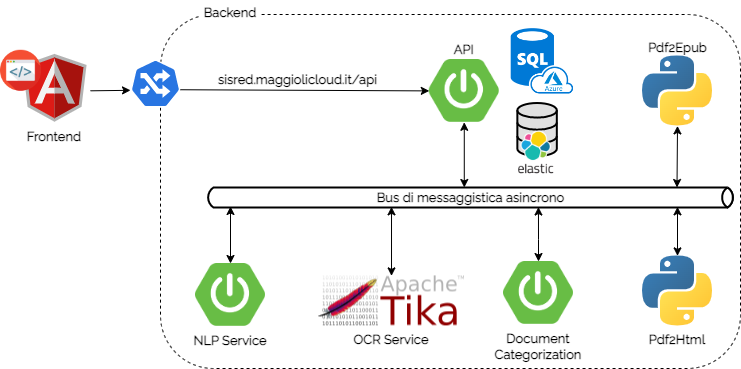
\includegraphics[width=1\textwidth]{img/tesi-7-sisred.drawio.png}
\caption{Architettura aggiornata del Sistema Redazionale}
\end{figure}
Attualmente il \textit{Sistema Redazionale} è installato su un cluster Kubernetes fornito \textit{as a Service} dal cloud provider Azure\footnote{\url{https://azure.microsoft.com/en-us/services/kubernetes-service/}}. Per effettuare il deploy dei vari componenti installati sul cluster è utilizzato \textit{Helm}\footnote{\url{https://helm.sh/}}, un tool open-source per effettuare templating di manifest Kubernetes e distribuire "pacchetti", chiamati \textit{chart}, nel mondo Kubernetes. Anche per il servizio \textit{pdf2epub} è adottato lo stesso meccanismo di deploy tramite l'installazione di un chart all'interno del cluster:
% TODO: descrivere helm chart utilizzato per deployare pdf2epub